% Gallery figure source
% Summary: Rooted and unrooted binary phylogenetic trees. In both cases the defining tree property is absence of cycles.
\documentclass[tikz,border=6pt]{standalone}
% Shared color palette
\usepackage[T1]{fontenc}
\usepackage[utf8]{inputenc}
\usepackage{lmodern}
\usepackage{microtype}
\usepackage{amsmath,amssymb,mathtools}
\usepackage{xcolor}
\usepackage{tikz}
\usetikzlibrary{arrows.meta,positioning,calc,fit,backgrounds,decorations.pathreplacing,shapes.geometric,shadows.blur}

\definecolor{mainblue}{RGB}{42,85,132}
\definecolor{deepgreen}{RGB}{30,105,70}
\definecolor{burntorange}{RGB}{190,90,25}
\definecolor{softgray}{RGB}{245,246,248}
\definecolor{darkgray}{RGB}{70,70,70}
\definecolor{violet}{RGB}{110,70,150}

\newcommand{\given}{\,|\,}
\newcommand{\Ne}{N_{e}}
\newcommand{\ARG}{\mathrm{ARG}}
\newcommand{\MRCA}{\mathrm{MRCA}}
\newcommand{\GMRCA}{\mathrm{GMRCA}}

% Shared TikZ styles
\tikzset{
  tip/.style={circle,fill=black,inner sep=1.6pt},
  nodept/.style={circle,fill=black,inner sep=1.4pt},
  sampled/.style={rectangle,fill=black,inner sep=2.2pt},
  branch/.style={line width=0.8pt},
  retic/.style={circle,draw=burntorange,fill=burntorange!25,line width=0.8pt,inner sep=2.0pt},
  event/.style={circle,draw=mainblue,fill=mainblue!15,line width=0.8pt,inner sep=1.8pt},
  arr/.style={-{Latex[length=2.0mm]},line width=0.8pt},
  faint/.style={line width=0.7pt,draw=gray!55},
  parentedge/.style={-{Latex[length=2.0mm]},line width=0.9pt,draw=burntorange},
  treeedge/.style={-{Latex[length=2.0mm]},line width=0.9pt,draw=black},
  segment/.style={line width=4pt,line cap=round},
  dashedretic/.style={-{Latex[length=2.0mm]},line width=0.9pt,draw=burntorange,dashed}
}


\begin{document}
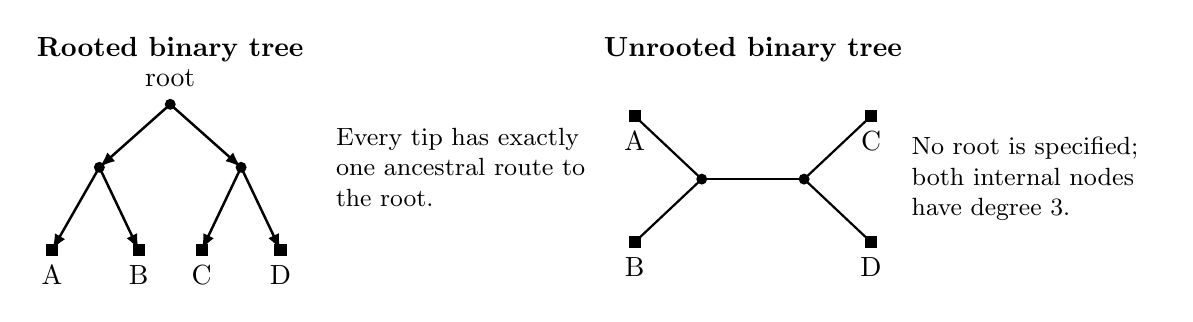
\begin{tikzpicture}[scale=1.0]
  \node[font=\bfseries] at (1.7,3.0) {Rooted binary tree};
  \begin{scope}[yshift=-0.25cm]
    \coordinate (r) at (1.7,2.55);
    \coordinate (n1) at (0.8,1.75);
    \coordinate (n2) at (2.6,1.75);
    \coordinate (a) at (0.2,0.7);
    \coordinate (b) at (1.3,0.7);
    \coordinate (c) at (2.1,0.7);
    \coordinate (d) at (3.1,0.7);

    \draw[treeedge] (r)--(n1);
    \draw[treeedge] (r)--(n2);
    \draw[treeedge] (n1)--(a);
    \draw[treeedge] (n1)--(b);
    \draw[treeedge] (n2)--(c);
    \draw[treeedge] (n2)--(d);

    \foreach \p in {r,n1,n2}{
      \node[nodept] at (\p) {};
    }

    \foreach \p/\lab in {a/A,b/B,c/C,d/D}{
      \node[sampled] at (\p) {};
      \node[below=2pt] at (\p) {\lab};
    }

    \node[above=3pt] at (r) {root};
    \node[right=8pt,text width=3.2cm,font=\small] at (3.4,1.75)
      {Every tip has exactly one ancestral route to the root.};
  \end{scope}

  \begin{scope}[xshift=7.4cm]
    \node[font=\bfseries] at (1.7,3.0) {Unrooted binary tree};

    \coordinate (uL) at (1.05,1.35);
    \coordinate (uR) at (2.35,1.35);

    \coordinate (ua) at (0.20,2.15);
    \coordinate (ub) at (0.20,0.55);
    \coordinate (uc) at (3.20,2.15);
    \coordinate (ud) at (3.20,0.55);

    \draw[branch] (uL)--(uR);
    \draw[branch] (uL)--(ua);
    \draw[branch] (uL)--(ub);
    \draw[branch] (uR)--(uc);
    \draw[branch] (uR)--(ud);

    \foreach \p in {uL,uR}{
      \node[nodept] at (\p) {};
    }

    \foreach \p/\lab in {ua/A,ub/B,uc/C,ud/D}{
      \node[sampled] at (\p) {};
      \node[below=2pt] at (\p) {\lab};
    }

    \node[right=4pt,text width=3.1cm,font=\small] at (3.45,1.35)
      {No root is specified; both internal nodes have degree 3.};
  \end{scope}
\end{tikzpicture}
\end{document}
